\section{Schema Components}
\label{sec:schema_def}
EL schemas are rich, hierarchical data structures composed primarily of a set of EL \textbf{formulas} organized into one of several disjoint, named \textbf{sections}.
Each formula has a section-dependent \textbf{formula ID} to uniquely identify it within the scope of the schema.
Each schema also has a \textbf{header}: an EL proposition, and an episode characterized by the proposition, which names and summarizes the entire schema. 
Each header has a unique verb predicate at its core, and its arguments are variables defined and typed within the scope of the schema.
The header can be used to ``embed'' a schema as a step in another schema---in fact, each step in Figure~\ref{fig:libschema} is a header for an embedded schema---or it can be matched directly to a proposition in a story to automatically invoke the schema.

\begin{figure}
    \centering
    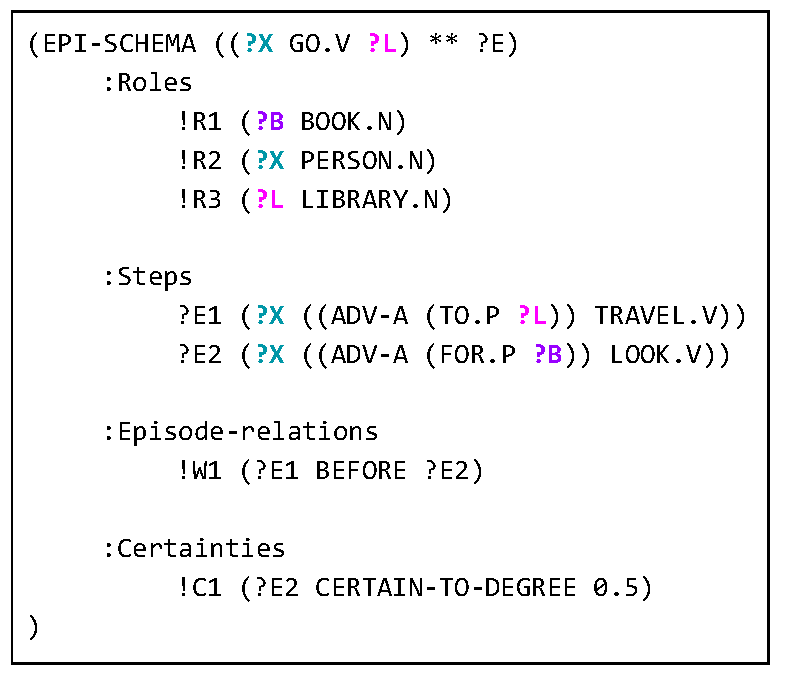
\includegraphics[width=0.65\columnwidth]{CH3_schemas/egschema.pdf}
    \caption{An example of a schema for a person going to a library.}
    \label{fig:libschema}
\end{figure}

\subsection{Formulas and Sections}
\label{sec:forms_secs}
% Introduce formulas and discuss their piecewiseness
% Introduce formula-section layout
Schemas organize their constituent formulas in two types of sections: \textit{fluent} and \textit{nonfluent} sections.
Nonfluent sections contain formulas that hold true regardless of time, and are marked by formula IDs beginning with exclamation marks.
Such formulas include type constraints on entities (Section~\ref{sec:roles}), temporal relation predications on episodes (Section~\ref{sec:eprels}), and equality constraints on variables within subordinate schemas (Section~\ref{sec:scoping}).
Fluent sections, on the other hand, contain formulas identified by variables starting with question marks; the truth value of these formulas is susceptible to change over time alone.
%Referring to the EL ontology in Figure~\ref{fig:el_ontology}, the semantic type of fluent predicates can be thought of as the more restrictive $(\mathcal{D}^{n} \rightarrow (\mathcal{M} \rightarrow \textbf{2}))$, rather than $(\mathcal{D}^{n} \rightarrow (\mathcal{S} \rightarrow \textbf{2}))$, as specific \textit{moments of time} ($\mathcal{M}$) are needed to determine truth value.
Referring to the EL ontology in Figure~\ref{fig:el_ontology}, the semantic type of fluent predicates can be thought of as $(\mathcal{D}^{n} \rightarrow (\mathcal{S'} \rightarrow \textbf{2}))$ , where $S'$ is a subset of situations whose elements temporally span only a single time point, as the predicate's truth value for given arguments may may vary from time point to time point.
Formally, a fluent formula $\phi$ with episode ID \el{?E} is said to characterize its episode ID: ($\phi ** \texttt{?E}$).
A non-fluent formula $\psi$, however, does not have an episode ID, as its truth value is not temporally constrained; instead, it is represented by a \textit{metavariable} \el{!M}, any occurrence of which in an EL formula may be equivalently \textit{replaced} with $\psi$.
Metavariables also exist for the characterizations ($\phi$ ** \el{?E}) implied by fluent formulas; a corresponding metavariable \el{!E} is introduced as a substitution representative for each such atemporal characterization formula.

\subsection{Steps and Temporal Relations}
\label{sec:steps}
EL schemas represent patterns of general, frequently co-occurring facts and events, the latter of which are primarily found within a schema's \el{:Steps} section.
The \el{:Steps} section is one of several fluent sections in a schema, and contains all of the events that may happen as a part of the schema.
Not all steps in a schema are required to happen---the \el{:Certainties} section allows expression of the probabilities of each step happening given that the schema as a whole happened.
Some schemas may have \textit{no} steps; such schemas are called \textit{atomic}, and exist to imbue the verb predicates in their header propositions with additional semantics, such as preconditions, postconditions, goals, and role constraints.
Most protoschemas (discussed in Section~\ref{sec:protoschemas}) are atomic.

Each step in a schema has a fluent episode ID \texttt{?Ei}, which the step formula implicitly characterizes.
Although the steps in a schema are linearized, they are not necessarily temporally sequential; the temporal model of EL allows for complex and explicit specification of temporal relations between events.
The \texttt{:Episode-relations} section contains two-place temporal predicates relating the schema's steps by their fluent IDs.
These temporal relations are taken from the Allen Interval Algebra \citep{allen1983maintaining}, under the simplifying assumption each step in the schema can be represented as a contiguous interval.

% steps of a schema are assumed to be linear unless eprels contradicts
% conjunctions are split up, XOR splits schema, splitting OR is OK depending on what semantics you want matching to have
% implicit relations to goals, preconds, postconds
% can embed other schemas (link to compo hierarchy)

\subsection{Roles}
\label{sec:roles}
% roles provide type and relational constraints on entities in the schema
% compare to other schema/DL frameworks and highlight relational constraints (OWL doesn't have rels, FN uses natural language)
% comparable to "semantic roles" in FN
% don't need to "declare" here to use a var in schema, but should probably be typed
The \texttt{:Roles} section of an EL schema contains nonfluent EL propositions meant to define the semantic roles of the variables used within the schema.
The propositions in the \texttt{:Roles} section may use monadic, often noun-based, predicates used to specify types, e.g. \el{(?B BOOK.N)} (\el{?B} \textit{is a book}), or they may use multi-argument predicates to relate entities to one another, e.g. \el{(?B PERTAIN-TO JOHN.NAME)} (\textit{book} \el{?B} \textit{belongs to John}).
%Role formulas provide a model-theoretic alternative to the natural language descriptions of semantic roles found in existing frame corpora like FrameNet and PropBank.
Because role formulas are concise, single-predicate EL propositions, they can function as individual predictions when a schema is matched to a formula parsed from a novel sentence: if an observed formula \el{(JOHN.NAME READ.V BIBLE1.SK)} matched to a schema formula \el{(?X READ.V ?B)}, the binding of \el{?B} to the individual \el{BIBLE1.SK} would also bind \el{?B} in the role formula \el{(?B BOOK.N)}, which leads to the standalone prediction \el{(BIBLE1.SK BOOK.N)} (\textit{``the Bible'' is a book}).

Role formulas may not always need to be satisfied exactly in order to conclude that a story has matched to a schema.
Because schemas are almost always tentative and the learning process is continual, a schema matching algorithm may want to allow a match even when an observed formula, e.g. \el{(NOT (OBJECT1.SK BOOK.N))}, directly contradicts a role formula, e.g. \el{(?B BOOK.N)}.
Non-equal predications, such as synonymic or hypernymic ones, may also be judged to satisfy the truth conditions of role predications for the purposes of schema matching.
These decisions are complex and depend on heuristics not easily renderable via model theoretic axioms, as we discuss in Section~\ref{sec:formal_semantics}.

%The \textbf{Roles} section of a schema is a \textit{nonfluent} section meant for putting ``eternal'' type constraints on the participating entities in the schema. All of the schema's variables, starting with question marks, can be viewed as Skolem functions of the schema's header episode, and they can be constrained in this section. In addition to type constraints, e.g. \texttt{(?X DOG.N)}, relational constraints between entities can also be specified in this section, e.g. \texttt{(?X PERTAIN-TO ?Y)}.

%In Figure~\ref{fig:protoschema}, the protoschema for movement from location to location, there are three main participating entities: \texttt{?X}, the agent doing the movement, and \texttt{?L1} and \texttt{?L2}, the source and destination locations. Those ``types'' are EL predicates, and are enforced by the predications in the protoschemas \textbf{Roles} section.

%When formulas are unified with a schema, these formulas are used as constraints for evaluating whether the individuals bound to the variables satisfy the schema's semantics. They are evaluated in a knowledge base populated by facts from the story, and potentially by formulas predicted from other confirmed schema matches. Partial matches, or matches with partial constraint satisfaction, can still be valuable: ``Breaking the mold'' of known schemas is part of the learning process. More detail on constraint evaluation and scoring will be given in Section~\ref{sec:scoring}.

\subsection{Preconditions, Postconditions, Goals, and Beliefs}
\label{sec:preconds}
% compare preconds and postconds to other schema systems
% motivate goals
% discuss chaining by pre/postcond unification
% discuss importance of mental state modeling
% discuss how EL reifiers let us model beliefs, etc.
Actions undertaken in the real world are frequently goal-driven, and a representation of how actions change the world and why characters might perform them is necessary to understand the story. The episodes characterized by the formulas in the precondition section are tacitly assumed to start before the schema's header episode (adjoining or overlapping it), and those characterized in the postcondition section extend beyond the header episode (post-adjoining or overlapping it).
%Schema matches can be ``chained together'' into composite, multi-step schemas by unifying their pre- and post-conditions, or their goals and post-conditions. An example of a learned ``chained'' schema is given in Figure~\ref{fig:eg_schema}.

\subsection{Temporal Relations}
\label{sec:eprels}
% enumerate temporal relations
% know what you're talking about with timegraph
Schemas characterize EL episodes that encompass their temporal duration. They also contain many other episodes, such as steps and preconditions, with their own temporal bounds. These episodes can all be complexly inter-related using constraints from the Allen Interval Algebra \citep{allen1983maintaining}. Pre- and post-conditions are implicitly constrained to be true at the start and end of the schema's header episode, respectively, and steps, by default, are ordered sequentially as listed in the schema, but additional constraints can be specified in the \textbf{Episode-relations} section of each schema. To evaluate these interval constraint propositions, we implemented a time graph specialist module \citep{gerevini1993efficient}.

\subsection{Scoping and Skolemization}
\label{sec:scoping}
% discuss dynamic skolemization
The header episode of each schema $\mathcal{S}$ characterizes a header episode, which we will refer to, without loss of generality, as \el{?E}. An EL schema's variables are not explicitly quantified in any of its formulas; instead, their values are implicitly given by a Skolem function of \el{?E}. We refer to the domain of the Skolem function, which is equal to the set of free variables in the schema, as the schema's \textit{scope}. Each compositionally nested schema $\mathcal{S}_{i}$, represented as step $\texttt{?E}_{i} \in steps(\mathcal{S})$, has its own Skolem function and its own scope; scope is not shared with a compositional parent schema unless explicitly bound in the \texttt{:Subordinate-constraints} section, or implicitly bound when unifying the parent schema's step formula for $\texttt{?E}_{i}$ with the header formula of $\mathcal{S}_{i}$.

The Skolem functions of schema $\mathcal{S}$, which characterizes episode \texttt{?E}, map variable names bound by $\mathcal{S}$ to values.
A \textit{Skolem mapping function} for $\mathcal{S}$, written as the symbol $\texttt{?E}\hspace{-2mm}\rightarrow$, can be applied to variable names to return the value of the Skolem function for that variable name within the scope of $\mathcal{S}$.
An example of this application is $(\texttt{?E}\hspace{-2mm}\rightarrow \el{?X})$, which evaluates the Skolem function for the variable \el{?X} within the scope of \el{?E}.
The reason that the Skolem mapping function uses the header episode name, \el{?E}, is to allow schemas that embed $\mathcal{S}$ using the episode \el{?E} to specify the exact instance of $\mathcal{S}$ to fetch Skolem functions for.
Likewise, the Skolem functions of each nested schema $\mathcal{S}_{i}$ can be written as $\texttt{?E}_{i}\hspace{-2mm}\rightarrow$. This notation may be used in the \texttt{:Subordinate-constraints} section of each schema to explicitly bind a variable in a nested schema's scope to one in the parent schema's scope, as seen in Figure~\ref{fig:compo_hier}.
